\documentclass{report}
\usepackage{listings}
\usepackage{graphicx}

\begin{document}
\title{Report 6 - Map}
\begin{figure}
    \centering
    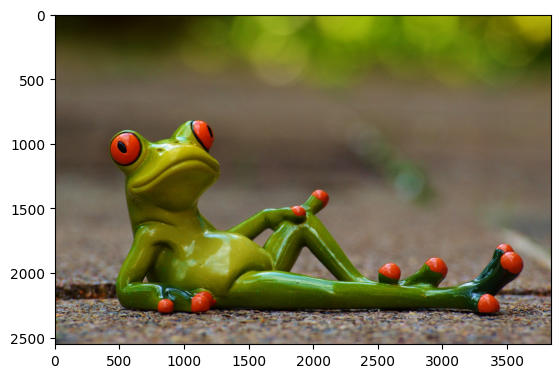
\includegraphics[width=1\linewidth]{base_frog_2D.png}
\end{figure}
\maketitle

\section{Introduction}
3 little kernels to implement.

\section{grayscale image binarization}
\begin{lstlisting}[language=Python]
@cuda.jit
def binarization(src, dst, threshold):
  # where are we in the input?
  x = cuda.threadIdx.x + cuda.blockIdx.x * cuda.blockDim.x
  y = cuda.threadIdx.y + cuda.blockIdx.y * cuda.blockDim.y

  if y < src.shape[0] and x < src.shape[1]:
    src[y, x] = [255 if src[y, x] > threshold else 0]
\end{lstlisting}

\section{brightness control}
This one takes an additional argument and will brighten or darken the image based on its value.
\begin{lstlisting}[language=Python]
@cuda.jit
def brightness_control(src, dst, value):
  # where are we in the input?
  x = cuda.threadIdx.x + cuda.blockIdx.x * cuda.blockDim.x
  y = cuda.threadIdx.y + cuda.blockIdx.y * cuda.blockDim.y
  if y < src.shape[0] and x < src.shape[1]:
    for i in range(3):
      dst[y, x, i]=min(255,(max(0,src[y, x, i]+value)))
\end{lstlisting}

Example: frog with +150 brightness
\newline
\begin{figure}[ht]
    \centering
    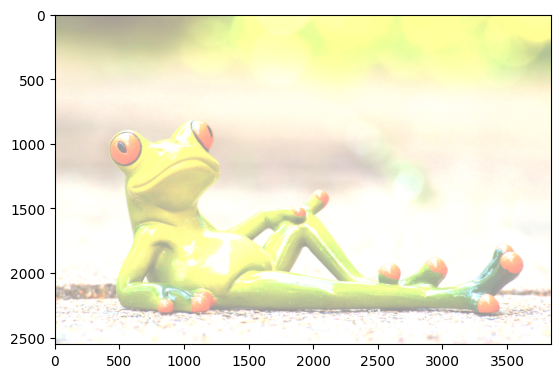
\includegraphics[width=1\linewidth]{bright_frog.png}
\end{figure}

\section{blending two images}
This one take a coefficient as an argument and will blend the 2 images given. The coefficient acts as the weight for the first image.
\begin{lstlisting}[language=Python]
@cuda.jit
def blend_images(src1, src2, q, dst):
  # where are we in the input?
  x = cuda.threadIdx.x + cuda.blockIdx.x * cuda.blockDim.x
  y = cuda.threadIdx.y + cuda.blockIdx.y * cuda.blockDim.y
  if y < src1.shape[0] and x < src1.shape[1]:
    for i in range(3):
      dst[y][x][i]=q*src1[y][x][i]+(1-q)*src2[y][x][i]
\end{lstlisting}
Example: the frog has a 0.6 coefficient, meaning the blobfish has 0.4
\begin{figure}[ht]
    \centering
    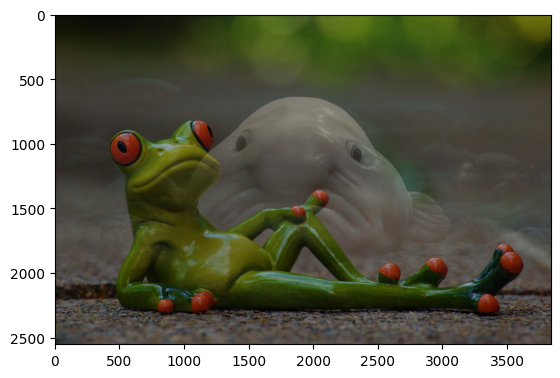
\includegraphics[width=1\linewidth]{blobfish_over_frog.png}
\end{figure}
\end{document}